\documentclass[fleqn,10pt,numbers]{olplainarticle}
\usepackage{float}
\usepackage{gensymb}
\usepackage{rotating}
\usepackage{booktabs}
\usepackage{graphicx}
\usepackage[labelfont=bf]{caption}
\usepackage{subcaption}
\usepackage{hyperref}
\usepackage{xcolor}
% Arabic script for the one-time introduction of the Rub' al-Khali (pdflatex).
% arabtex redefines \begin so that every environment, including document,
% opens a group; restore LaTeX's \begin/\end after loading it.
\let\LaTeXbegin\begin \let\LaTeXend\end
\usepackage{arabtex}
\usepackage{utf8}
\setcode{utf8}
\let\begin\LaTeXbegin \let\end\LaTeXend
\newcommand{\todo}[1]{\textcolor{red}{\textbf{[TODO: #1]}}}
\hypersetup{hidelinks}

\title{Landscape-scale bacterial biogeography across the Rub' al-Khali}

\author[1]{Rund Tawfiq}
\author[1]{Marwa Abdelhakim}
\author[3]{Sulaiman M. Alajel}
\author[1]{Mohammed Alarawi}
\author[8]{Hind Aldakhil}
\author[1]{Abderahmane Derouiche}
\author[5]{Daniela I. Drautz-Moses}
\author[4]{Michel Dumontier}
\author[7]{Raik Grünberg}
\author[1]{Alejandra Lopez-Velazquez}
\author[2]{Susana Martinez Arbas}
\author[1]{Kexin Niu}
\author[1]{Krishnakumar Sivakumar}
\author[6]{Tiannyu Wang}
\author[5]{Xiang Zhao}
\author[1]{Jood Zubair}
\author[6]{Magnus Rueping}
\author[1]{Robert Hoehndorf\thanks{Correspondence:
  robert.hoehndorf@kaust.edu.sa}}
%% ORCIDs received from co-authors (August 2026), for the submission system;
%% the olplainarticle class has no ORCID field.
%%   Daniela I. Drautz-Moses    0000-0002-3739-0917
%%   Susana Martinez Arbas      0000-0001-7309-8190
%%   Alejandra Lopez-Velazquez  0009-0001-2873-5311
%%   Xiang Zhao                 0009-0007-8662-9406
%%   Jood Zubair                0009-0005-9532-0801
%%   Abderahmane Derouiche      0000-0002-3241-1424
%%   Kexin Niu                  0000-0002-7302-0462
%%   Hind Aldakhil              0000-0001-9491-103X
%%   Michel Dumontier           0000-0003-4727-9435
%%   Raik Grünberg              0000-0001-9532-6043
%%   Robert Hoehndorf           0000-0001-8149-5890

\affil[1]{Bio-Ontology Research Group (BORG), Computer, Electrical and
  Mathematical Sciences and Engineering (CEMSE) Division, King Abdullah
  University of Science and Technology (KAUST), Thuwal, Saudi Arabia}
\affil[2]{NIUM, Esch-sur-Alzette, Luxembourg}
\affil[3]{Ministry of Environment, Water and Agriculture, Saudi Arabia}
\affil[4]{Institute of Data Science, Department of Advanced Computing
  Sciences, Faculty of Science and Engineering, Maastricht University,
  Maastricht, The Netherlands}
\affil[5]{Bioscience Core Lab, King Abdullah University of Science and
  Technology, Thuwal, Saudi Arabia}
\affil[6]{Physical Science and Engineering (PSE) Division, King Abdullah
  University of Science and Technology (KAUST), Thuwal, Saudi Arabia}
\affil[7]{Biomedical Sciences Division (BioMed), King Abdullah University of Science and Technology (KAUST),
  Thuwal, Saudi Arabia}
\affil[8]{National Livestock \& Fisheries Development Program (NLFDP),
  Ministry of Environment, Water and Agriculture (MEWA), Riyadh 13413,
  Saudi Arabia}

\keywords{Rub' al-Khali, Empty Quarter, hyperarid soil microbiome, bacterial
  biogeography, landscape-scale survey, spatiotemporal, repeated sampling, $16$S
  rRNA amplicon survey}

\begin{abstract}
The Rub' al-Khali (Empty Quarter) is the world's largest continuous sand desert, yet the
bacterial ecology of its open Saudi interior has not been surveyed. We present
the first landscape-scale bacterial survey of this region, with $5$
expeditions to $60$ sites over $31$ months and paired surface, shallow-subsurface,
and root-adjacent soil. Bacterial communities formed a recurring geographic
pattern: distant sites contained more different communities, mainly because
taxa replaced one another across the landscape. Within sites, root-adjacent
communities were distinct and less even than both bulk soil compartments, showing
that local soil context changes which bacteria dominate. Long-term temperature,
rainfall, and humidity tracked diversity and the relative abundance of many
genera, while richness showed a short positive association with recent rainfall,
strongest during the first several days. Soil pH accounted for part of the
geographic pattern. The metabolic pathways predicted from the $16$S sequences
retained both geographic and compartment structure, and their broad
gene-family profiles agreed with matched shotgun data. Checks for DNA from
damaged cells and for low-biomass contamination showed that these possible
assay effects did not change the main ecological conclusions. The study
establishes a regional biological baseline
and a reusable resource for biodiversity monitoring, restoration,
arid-agriculture research and evidence-based land planning.
\end{abstract}

\begin{document}

\flushbottom
\maketitle
\thispagestyle{empty}

%% ====================================================================
\section*{Introduction}
%% ====================================================================

The Rub' al-Khali (Arabic \RL{الربع الخالي}; in English, the Empty Quarter)
is the world's largest continuous sand
desert. It covers much of the southern Arabian Peninsula, mainly within Saudi
Arabia \cite{edgell2006arabian}, and shapes land use, conservation, and plans for
agriculture across the region. Yet the bacteria in its open interior have not
been surveyed. The closest molecular community study examined a
groundwater-fed salt flat in the United Arab Emirates, a habitat unlike the
open sand soils of the Saudi interior \cite{mckay2016sabkha}. A regional survey
is needed both to understand this major desert and to provide a reference for
future monitoring, restoration and arid-land research.

Work in other deserts shows why such a survey matters. Dry landscapes that look
uniform can contain strong changes in bacterial composition. Climate, soil pH,
salts and minerals are often associated with these changes
\cite{fierer2006toward,delgadobaquerizo2018global,maestre2015increasing,
shen2021atacama}. Rare rainfall can also trigger a short biological pulse before
the soil dries again \cite{noymeir1973desert,schwinning2004pulse}. Sampling
sites at different delays after rainfall can therefore test whether diversity rises
and then declines, although it cannot identify the process. One visible
spatial outcome is distance decay: nearby sites contain more similar
communities than distant sites
\cite{nekola1999distance,hanson2012biogeography,bay2020negev}. This pattern can
arise because taxa replace one another across the landscape, or because poorer
communities become subsets of richer ones. Replacement implies distinct local
assemblages; nestedness implies loss from a shared pool. Neither process has
been measured across the open Empty Quarter.

Desert soil can also change within centimetres. The surface receives direct
sunlight and strong heating, while soil at $5$--$10\,\mathrm{cm}$ is partly buffered \cite{horstmann2024atacama}. Sparse
plants may add water and carbon near their roots
\cite{eida2018desertplants,maurice2023fertility}. These
differences can change which taxa occur, which taxa dominate, and which
metabolic pathways the community is predicted to encode. Richness alone cannot
separate these
outcomes: two soils may contain similar numbers of taxa while their abundance
and predicted functional profiles differ. DNA can also remain after cells die.
This relic DNA, together with contamination introduced during laboratory
processing, is a particular concern in low-biomass desert soil. Biological
interpretation therefore requires controls that distinguish these sources of
DNA from the sampled community \cite{fierer2025controls}.

Surveys elsewhere on the Arabian Peninsula have described bacteria along elevation gradients, at single
arid locations, and in plant-associated soil
\cite{yasir2015elevation,khan2020saudi,osman2016jizan,eida2018desertplants,
jalal2022saudi,maurice2023fertility,maurice2024alula}. None covers the open
Empty Quarter at landscape scale or combines a dense transect with repeated
sampling of several compartments. We therefore sampled $60$ sites during $5$
expeditions over $31$ months. We asked how bacterial composition changes across
the landscape and among compartments; how climate, pH and elemental
composition relate to those patterns; whether predicted metabolic potential
changes with them; and whether relic-DNA and low-biomass controls alter the
main conclusions. The resulting survey maps bacterial biogeography at landscape and centimetre scales, with the samples, measurements, sequences, and their production records preserved as a linked resource for reuse \cite{rubalkhali_datapaper}. Communities form a recurring geographic mosaic in which taxa replace one another across the sand sea. Within a site, the compartment (surface, shallow-subsurface or root-adjacent soil) changes which taxa dominate rather than how many taxa are detected. Long-term climate and soil pH track the geographic pattern. Richness shows a short positive association with recent rainfall, and predicted metabolic potential retains both spatial structures; neither the relic-DNA nor the low-biomass controls change these conclusions.

%% ====================================================================
\section*{Results}
%% ====================================================================

\subsection*{Bacterial communities change across the landscape}

We surveyed 60 sites along a west--east transect through the Saudi
Empty Quarter and returned during 5 expeditions over 31 months
(Figure~\ref{fig:landscape}a). At each visit, we sampled bulk surface soil,
bulk subsurface soil (``deep'' soil), and root-adjacent soil, collecting three replicates per compartment. We sequenced the V3--V4 marker region of the bacterial 16S rRNA gene and
resolved the reads into amplicon sequence
variants (ASVs). This yielded $1{,}237$ quality-controlled profiles, of which $1{,}227$ come from the repeatedly sampled sites 1--60 (Figure~\ref{fig:landscape}b). Trip~$2$ covered
only 8 sites due to extreme heat. Supplementary Table~S1 lists the
samples used in each analysis.

Eight phyla each held more than $2\,\%$ of reads on average across the
$1{,}227$ core-site profiles: Pseudomonadota ($26.9\,\%$), Bacillota
($22.5\,\%$), Actinomycetota ($18.7\,\%$), Chloroflexota ($8.6\,\%$),
Bacteroidota ($7.1\,\%$), Planctomycetota ($3.2\,\%$), Gemmatimonadota
($2.7\,\%$) and Acidobacteriota ($2.3\,\%$); Cyanobacteriota held
$0.4\,\%$ (Supplementary Section~S5.6). Bacilli was the leading class
($21.0\,\%$), ahead of Gammaproteobacteria ($14.7\,\%$), Actinobacteria
($13.3\,\%$) and Alphaproteobacteria ($12.2\,\%$). The leading genera were
\textit{Domibacillus} ($6.2\,\%$ of reads), \textit{Massilia} ($3.5\,\%$),
\textit{Bacillus} ($3.0\,\%$), \textit{Microvirga} ($2.4\,\%$) and
\textit{Flavisolibacter} ($2.0\,\%$), followed by
\textit{Noviherbaspirillum}, \textit{Streptomyces}, \textit{Herpetosiphon},
\textit{Paenibacillus} and \textit{Lysinibacillus}; \textit{Domibacillus}
led every compartment. Endospore-forming Bacillota and Actinomycetota therefore
supplied over $40\,\%$ of reads, whereas Acidobacteriota and
Verrucomicrobiota, which rank among the most abundant phyla in global soil
surveys \cite{delgadobaquerizo2018global,fierer2017embracing}, together held
$3.3\,\%$. These shares describe the marker-gene profile, not cell counts.

We investigated whether community composition changed gradually across the
sampled transect. The model allowed two broad patterns: a steady change from west to east,
or a smooth change in its rate that could reverse direction once. These were
represented by a straight-line term and a squared-location term. Together,
these patterns accounted for $40.2\,\%$ of the site-averaged difference in
relative taxon abundance across $630$ site, expedition, and compartment
combinations ($95\,\%$ CI, $32.5$--$47.8\,\%$; $p=0.001$).
The result remained when we changed the number of genera, used ASVs as the taxonomic units,
or omitted any one expedition
(Supplementary Section~S5.3). The geographic pattern therefore did not depend
on grouping sequences into genera or on a single visit.

Communities also became less similar with distance. We therefore asked a more
direct question: did sites farther apart have
more different relative taxon abundances? We measured this with Aitchison
dissimilarity, which compares the ratios among taxa rather than raw read
totals. It is zero when two relative compositions are identical and increases
as their taxon ratios diverge \cite{gloor2017compositional}. A positive slope
with distance therefore shows how rapidly community composition changes across
the landscape. The slope was $1.351$ ($95\,\%$ CI, $0.905$--$1.796$), $1.510$
($1.092$--$1.929$) and $1.180$ ($0.698$--$1.662$) dissimilarity units per
$100\,\mathrm{km}$ in surface, shallow-subsurface and root-adjacent soil, respectively
(each $p=0.0001$; Figure~\ref{fig:landscape}c). The slopes differed among
compartments ($p=0.0053$): composition changed fastest below the surface and
slowest next to roots.

Finally, we asked what kind of change produced these differences. After
comparing every sample at the same read coverage, we used Sørensen
dissimilarity to compare the proportions of shared and unshared taxa between
two sites. It is zero for identical taxon lists and increases as fewer taxa are
shared. We separated taxa
that replaced one another between sites from taxa lost from an otherwise
shared pool; these components are called turnover or replacement and nestedness,
respectively \cite{baselga2010partition}. Replacement represented 
$69$--$75\,\%$ of the average difference in every compartment. Both components
rose with distance, but replacement dominated. The Empty Quarter is therefore
a mosaic of distinct bacterial assemblages rather than a simple decline from
one shared community.

The replacement had identifiable participants. Among the $200$ genera of the
route model, $124$ changed monotonically along the route after correction for
the $200$ tests: $77$ declined from west to east and $47$ increased
(Supplementary Section~S5.6). The declining genera were mostly Actinomycetota
($27$ of $77$; for example \textit{Cellulomonas}, Spearman $\rho=-0.79$,
\textit{Marmoricola} and \textit{Streptomyces}), Pseudomonadota ($20$;
\textit{Sphingomonas}, \textit{Steroidobacter}, \textit{Massilia}),
Bacteroidota ($9$) and Acidobacteriota ($4$; \textit{Blastocatella},
\textit{Aridibacter}). The increasing genera were led by Bacillota ($17$ of
$47$): \textit{Bacillus} rose from $1.6$ to $6.2\,\%$ of reads between the
western and eastern thirds ($\rho=0.77$) and became the leading genus of the
eastern third, joined by genera typical of saline and alkaline soils such as
\textit{Halalkalibacter} ($\rho=0.85$), \textit{Halomonas},
\textit{Aquibacillus} and \textit{Pseudalkalibacillus}. The eastern sites are
also the warmer, more humid and more alkaline end of the route (site means:
Spearman $\rho$ with route position $0.98$ for temperature, $0.92$ for humidity
and $0.82$ for pH), so these genera mark the environmental gradient without
identifying its cause.

\begin{figure}[!htbp]
\centering
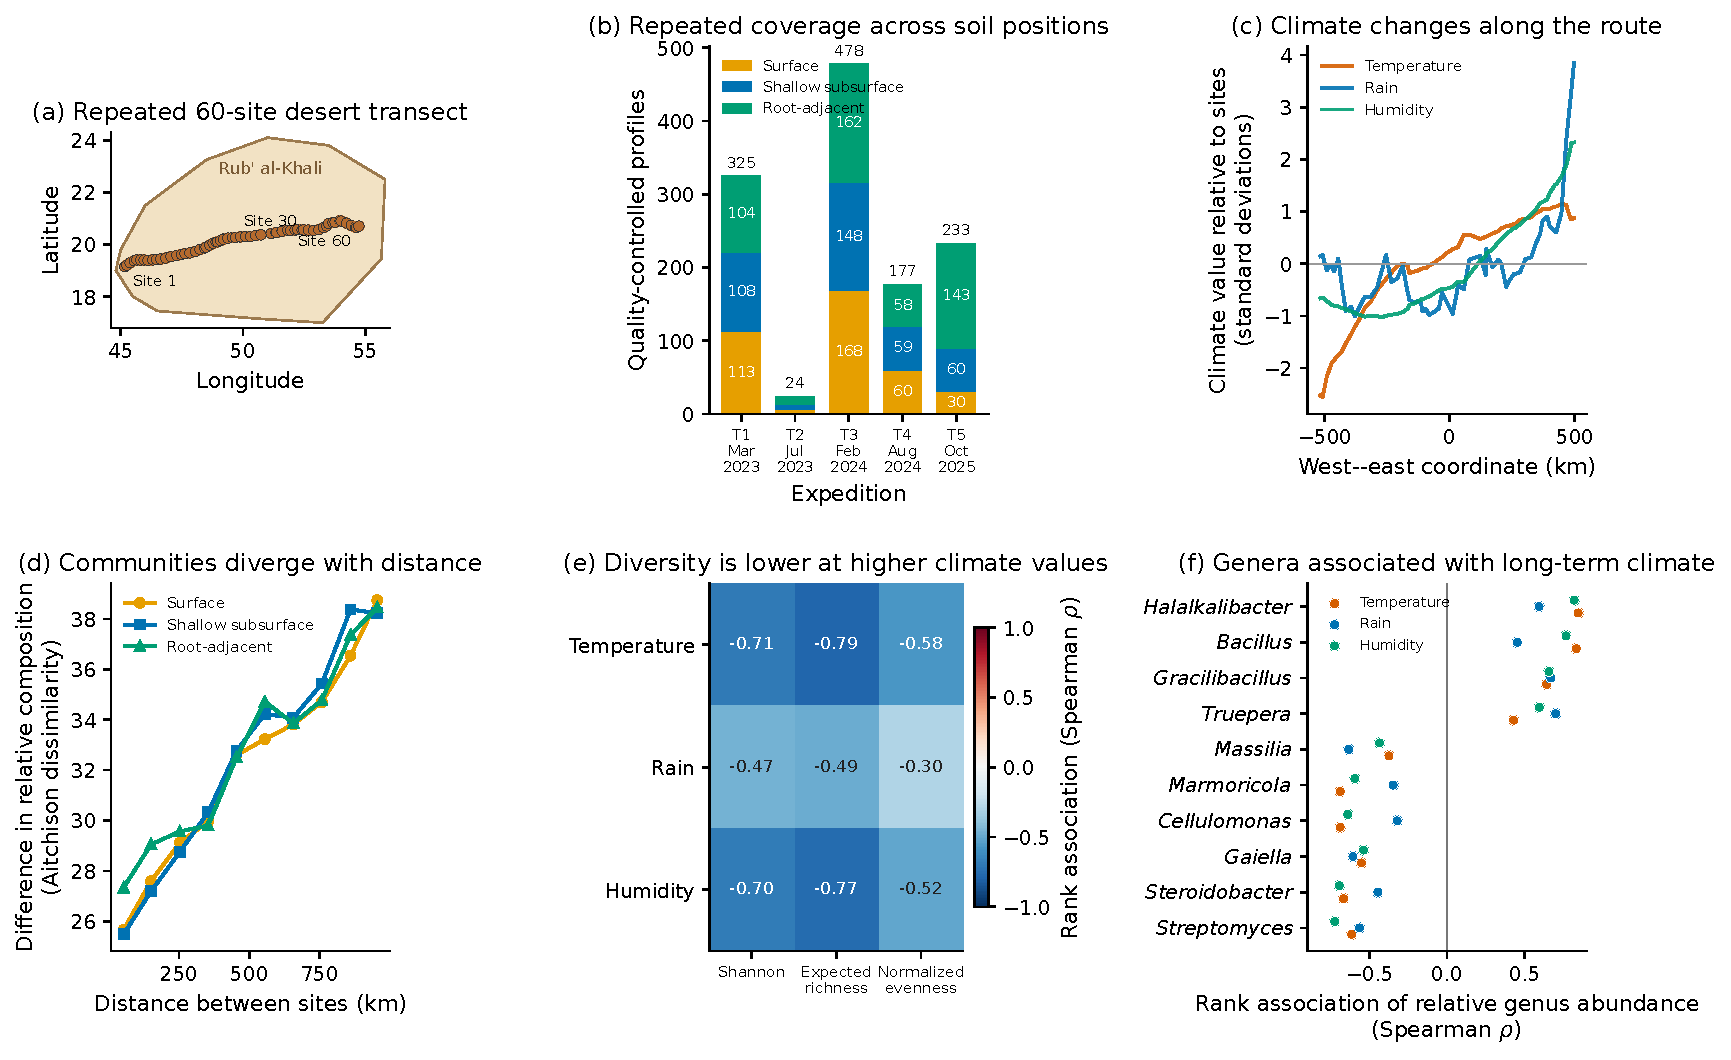
\includegraphics[width=\linewidth]{figures/fig1_landscape.pdf}
\caption{Survey design, geographic differences and climate associations.
  (a) The $60$ core sites along the west--east route on a NASA Blue Marble
  satellite image (July 2004); the dashed outline marks the Empty Quarter
  boundary for orientation only. (b) The $1{,}237$ quality-controlled profiles
  by expedition and compartment. Trip~$2$ reached $8$ sites. (c) The difference
  in relative community composition, measured as mean Aitchison dissimilarity,
  as distance between sites increases. The statistical test kept all
  comparisons involving the same site together. (d) Each site's $49$-month
  climate mean, expressed as standard deviations from the mean across all
  sites. (e) Rank associations between climate and diversity.
  Values near $-1$ mean that diversity consistently decreases as the climate
  variable increases; values near zero mean no consistent order. (f) The
  strongest supported genus associations. Tests in (e,f) were corrected for
  the number of comparisons.}
\label{fig:landscape}
\end{figure}

\subsection*{Compartment shapes bacterial composition and evenness}

We next asked whether compartment changed the relative abundance of taxa
within the same site and expedition. Across $170$ site-by-expedition
comparisons in which all three compartments were available, the separation
among the three average compositions was large relative to the variation
within compartments. This ratio is the pseudo-$F$ statistic: a larger value means
stronger overall separation. The compartment separation had
pseudo-$F=17.28$ ($p=0.001$).
We then asked whether sites shifted in a
consistent direction for each compartment pair. We divided the magnitude of the
average shift by the average magnitude of the individual site shifts. This
standardized displacement is near $1$ when sites shift in the same direction
and near $0$ when their shifts cancel. Root-adjacent and shallow-subsurface
soil showed the most consistent shift ($0.478$), followed by root-adjacent and
surface soil ($0.433$) and shallow-subsurface and surface soil ($0.331$;
Figure~\ref{fig:soil-position}a). All $3$ comparisons passed correction for
the $3$ tests and remained supported after changing the included
taxa, the treatment of zero counts, or the omitted expedition
(Supplementary Section~S5.1).

Shannon diversity combines the number of taxa with the balance of their read
abundances. It was lower in root-adjacent than shallow-subsurface soil by
$0.206$ on average (Figure~\ref{fig:soil-position}b). After resampling whole
sites, the $95\,\%$ interval was [$-0.398$,$-0.001$]. The difference remained
after adjustment for
sequencing depth and recorded extraction method ($-0.273$, $95\,\%$ CI
[$-0.424$,$-0.122$]).

To find what produced this change, we estimated how many taxa would be expected
if every profile had $25{,}000$ reads. We then scaled Shannon diversity by this
common-depth richness to separate the balance among taxa from their number.
This measure is normalized evenness: a high value means that reads are spread
across taxa, whereas a low value means that a few taxa dominate.
Evenness declined from shallow-subsurface to surface and then to root-adjacent
soil (Figure~\ref{fig:soil-position}c). Root-adjacent soil was lower than
surface soil by $0.0315$ ($95\,\%$ CI [$-0.0448$,$-0.0186$]) and lower than
shallow-subsurface soil by $0.0440$ ([$-0.0572$,$-0.0313$]). Expected richness
did not show the same order. Compartment therefore changed which taxa
dominated more consistently than it changed how many taxa were detected.
Because the read abundances are relative, we compared each genus with the
geometric mean abundance across all genera on a logarithmic scale. This avoids
treating the reads as absolute cell counts. The largest descriptive genus
shifts involved contrasts such as
\textit{Pelagibacterium}, \textit{Bradyrhizobium}, \textit{Deinococcus} and
\textit{Planococcus} (Figure~\ref{fig:soil-position}d). These values locate the
genera that contributed most to the overall composition difference; they do
not test each genus separately.

\begin{figure}[!htbp]
\centering
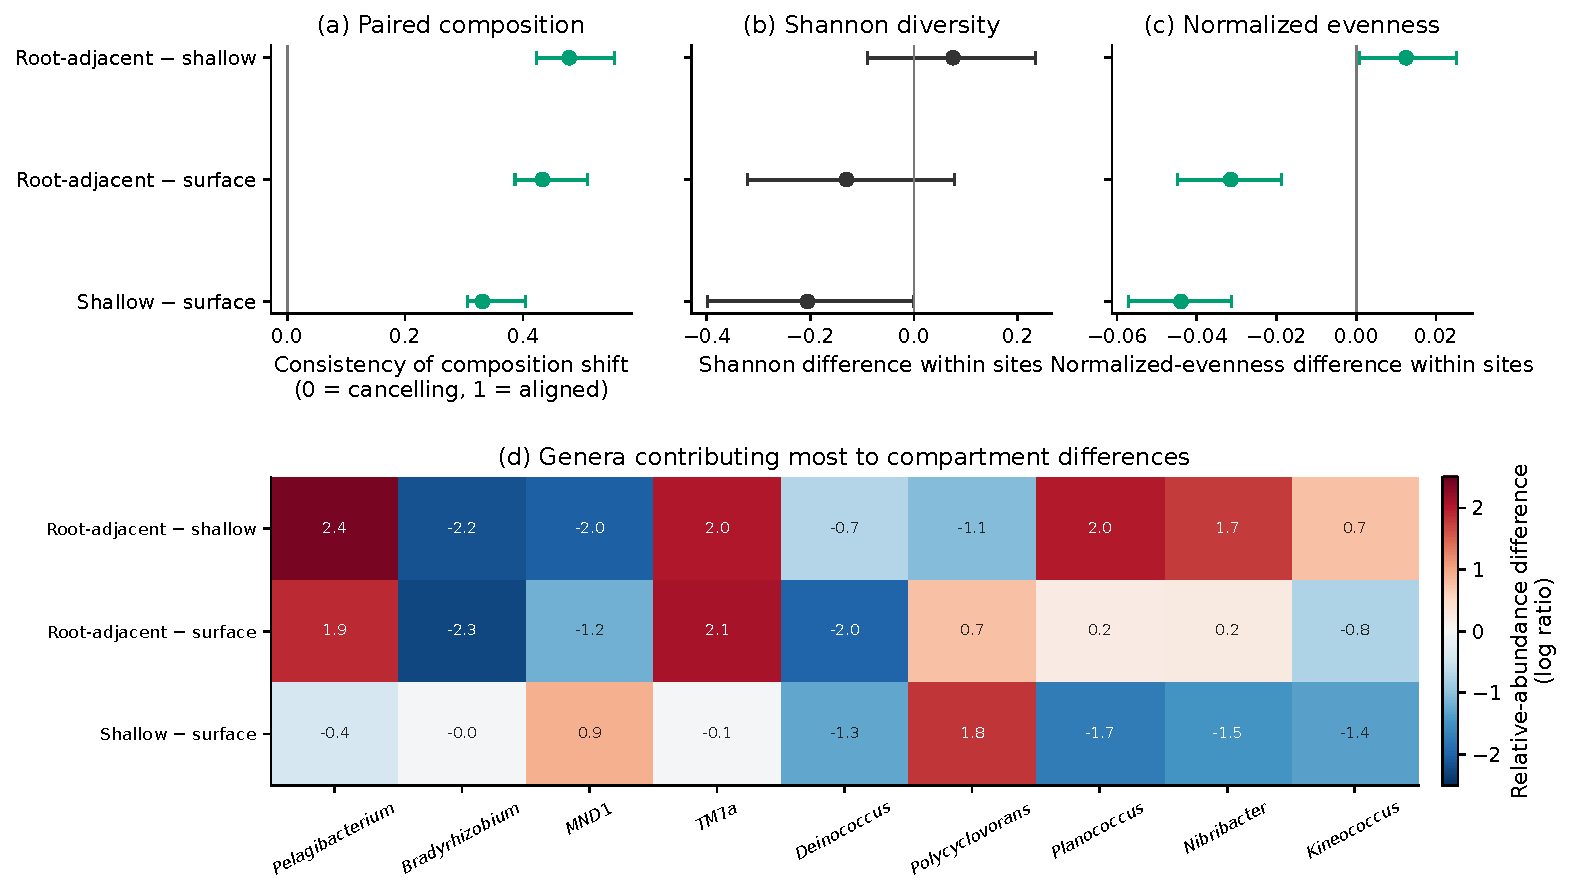
\includegraphics[width=\linewidth]{figures/fig2_soil_position.pdf}
\caption{Compartment differentiates bacterial communities within sites.
  (a) The consistency of the shift in relative taxon abundance across sites.
  Values approach one when sites shift in the same direction and zero when
  shifts cancel. (b,c) Paired differences in Shannon diversity and
  normalized evenness, averaged across expeditions. In (a--c), points show
  means and bars show $95\,\%$ intervals. (d) Genera that contributed most to the $3$ overall
  composition differences. Positive values mean a higher relative abundance
  in the first named compartment. This panel describes contributions to the
  overall difference and does not test genera separately.}
\label{fig:soil-position}
\end{figure}

\subsection*{Climate and soil properties track bacterial variation}

We recorded air temperature, pressure and relative humidity during $247$,
$177$ and $239$ quality-controlled site visits. Air temperature ranged from
$20.0$ to $49.4\,^{\circ}\mathrm{C}$ and humidity from $9.5$ to
$62.5\,\%$. To describe background climate rather than conditions at one
visit, we also summarized $49$ months per site from January $2022$ to January
$2026$. Long-term site means ranged from $26.38$ to
$30.30\,^{\circ}\mathrm{C}$, $1.31$ to $7.47\,\mathrm{mm}$ rainfall per month,
and $24.27$ to $35.40\,\%$ relative humidity. Figure~\ref{fig:landscape}d
shows how these site means changed across the transect.

We compared $3$ aspects of diversity: Shannon diversity combines taxon number
and abundance balance, expected richness estimates how many taxa would be
detected at a common read coverage, and normalized evenness measures how evenly
reads are spread after accounting for richness. We then asked whether sites
ordered from lower to higher climate values also showed a consistent order in
each. Spearman rank correlation measures this ordering: a value near $-1$ means
that diversity consistently decreases as the climate value increases, whereas a
value near zero means no consistent order. All $3$ long-term gradients tracked
all $3$ measures. Sites with higher temperature, rainfall and humidity had lower
Shannon diversity (Spearman $\rho=-0.71$, $-0.47$ and $-0.70$), lower expected
richness ($-0.79$, $-0.49$ and $-0.77$), and lower evenness ($-0.58$, $-0.30$
and $-0.52$) (Figure~\ref{fig:landscape}e). All $9$ associations remained supported after correction for the
$9$ comparisons (adjusted $p\leq0.021$). Among $200$ genera detected in at
least $20\,\%$ of profiles, $112$, $112$ and $111$ were associated with
temperature, rainfall and humidity after multiple-testing correction (Figure~\ref{fig:landscape}f).
The strongest positive associations with temperature were
\textit{Halalkalibacter}, \textit{Bacillus}, \textit{Pannonibacter},
\textit{Ammoniphilus} and \textit{Rhodocista} ($\rho=0.74$--$0.85$), and the
strongest negative associations were \textit{Cellulomonas},
\textit{Marmoricola}, \textit{Steroidobacter}, \textit{Ellin6055} and
\textit{Pseudonocardia} ($\rho=-0.65$ to $-0.69$); \textit{Streptomyces} had
the strongest negative association with humidity ($\rho=-0.73$). Because
climate covaries with location along the route, these are the genera that mark
the west--east replacement described above.
Supplementary Section~S7 gives the genus rankings and shows how strongly these
climate patterns overlap with location.

Quality-controlled pH measurements matched $702$ profiles and had a mean pH of
$7.986$.
After accounting for expedition and compartment, location along the route
explained $84.6\,\%$ of pH variation ($p\leq0.001$). Among the same $702$ matched
profiles, the share of bacterial composition explained by location fell from
$35.8\,\%$ to $19.6\,\%$ after pH adjustment. Excluding the group with the
highest pH, or its entire site, gave $18.7$--$19.6\,\%$. pH and location therefore
described substantial overlapping variation.

X-ray fluorescence (XRF) measured $11$ elements in at least $75\,\%$ of $725$ specimens.
Because the elements changed together, we combined them into one summary
gradient that captured the largest shared change. This gradient represented
$39.2\,\%$ of the elemental variation and a smaller but consistent share of
bacterial composition, $0.358\,\%$ ($p=0.010$). Planned changes to the included
taxa and treatment of zero values
gave estimates from $0.311$ to $0.543\,\%$ (Supplementary Sections~S2--S3). This
range shows sensitivity to analysis choices; it is not a confidence interval.

\subsection*{Bacterial richness shows a short association with recent rainfall}

We next asked whether rare rainfall was followed by a temporary rise in diversity.
The expeditions ran on fixed dates, so we could not sample before and after
individual storms; each sample was instead collected an incidental number of
days after the last rainfall at its site, and the delay at which any response
peaks was unknown. For each sample we therefore weighted rainfall over the
preceding $60$ complete days by a curve that rises to a maximum at day $p$ and
then decays, so that rainfall $p$ days before collection carries the most
weight. We scanned $p$ from $0.5$ to $30$ days across $3$ diversity measures
($180$ candidate models) while accounting for site, compartment, expedition
and location along the route, and retained the strongest positive association.

Retaining the best of $180$ results inflates significance, so we calibrated the
complete search rather than any single model. We rotated each expedition's
$60$-day rainfall series in a circle $19{,}999$ times, independently within
expeditions. Each rotation preserves the amount, rarity and clustering of rainfall
and its spatial pattern across sites, and breaks only its timing relative to
collection; because rotation acts within an expedition, it does not require
storms to recur across expeditions. Re-running the entire scan on every
rotation gave the distribution of the largest statistic obtainable when rainfall
timing is uninformative, against which we tested the observed result.

Expected richness was the selected endpoint in both daily rainfall products.
With NASA POWER, the primary series \cite{nasa_power_2024}, each additional
millimetre at the fitted peak was associated with $179.6$ additional expected
taxa ($95\,\%$ site-clustered CI, $92.1$--$267.1$); the fitted peak was $2$
complete days ($95\,\%$ peak-selection interval, $1.5$--$4.5$ days), rainfall
accounted for $3.64\,\%$ of the remaining variation ($0.60$--$7.87\,\%$), and
the family-wise one-sided test for a positive pulse gave $p=0.0560$.
Open-Meteo, an independent product \cite{openmeteo}, selected the same
endpoint with a peak at $1$ day ($0.5$--$6.5$ days), a larger estimate of
$327.5$ taxa per millimetre ($141.1$--$514.0$), $3.84\,\%$ explained variation
($0.57$--$8.99\,\%$), and $p=0.0432$ after the same correction. The two
products therefore agree on an early positive association but differ in its
size and exact timing (Supplementary Figure~S1).

Three checks bound this result. The pulse curve assumes a smooth rise and
decline; fitting rainfall from $7$ non-overlapping periods before collection
instead, with no assumed shape, placed the largest positive estimate at
$3$--$4$ days in both products. Rain falling after collection, which cannot
have an effect, produced no comparable pattern (largest richness statistic
$0.055$). The association was positive in every compartment and changed
little after accounting for pH, but weakened when the model allowed more
complex geographic change. Removing candidate contaminants also left the
estimate essentially unchanged, although its corrected probability then
crossed the conventional threshold ($p=0.0485$); we therefore do not use
filtering to strengthen the effect. The data support an early association
between rainfall and richness, not an exact delay or a causal mechanism
(Supplementary Section~S7).

\subsection*{Predicted metabolic pathways follow geography and compartment}

We used PICRUSt2, which compares each $16$S sequence with reference genomes, to
predict which metabolic pathways the community could encode
\cite{douglas2020picrust2}. These estimates describe metabolic potential, not
activity. Across $1{,}227$ core-site profiles and $462$ pathways in the
MetaCyc database \cite{metacyc}, the predicted profiles were dominated by
housekeeping metabolism. Biosynthesis pathways held $66.8\,\%$ of predicted
pathway abundance, energy and central metabolism $17.2\,\%$ and degradation or
utilization pathways $10.7\,\%$ (keyword classes; Supplementary
Section~S8.1). Aerobic respiration through cytochrome $c$ was the most
abundant single pathway ($1.7\,\%$), followed by branched-chain amino acid
and fatty acid biosynthesis. Carbon fixation was minor: the
Calvin--Benson--Bassham cycle ranked $44$th ($0.6\,\%$) and the reductive TCA
cycle $122$nd ($0.4\,\%$), in line with the $0.4\,\%$ read share of
Cyanobacteriota; the MetaCyc set used by PICRUSt2 contains no light-reaction
pathway. The predicted potential therefore describes an aerobic, heterotrophic
community rather than a phototroph-dominated crust. Against this shared
background, the $200$ most abundant pathways retained a strong geographic
pattern.
The same route model, which allowed the rate of change to vary smoothly and
reverse once, accounted for $23.4\,\%$ of the difference among site-level
pathway profiles ($95\,\%$ CI, $15.5$--$31.4\,\%$; $p=0.0001$). The result
remained supported after changing the included pathways, the treatment of zero
values, or the omitted expedition.

We then asked whether predicted pathway profiles differed among
compartments, and found a difference across $172$ complete site-by-expedition
comparisons ($p=0.0001$). We used the same standardized displacement as for
taxonomic composition. Predicted pathways shifted most consistently between
root-adjacent and shallow-subsurface soil ($0.453$) and between root-adjacent
and surface soil ($0.429$; both adjusted $p=0.00015$ after correction for $3$
comparisons; Figure~\ref{fig:function-controls}a). Of $600$ tests covering
$200$ pathways and $3$ compartment pairs, $270$ remained supported after
correction. They included pathways for amino acids, cofactors, carbohydrates
and cell envelopes; Supplementary Section~S8.1 gives the complete results.

From west to east along the transect, $2$ pathways that produce the fatty
acids cis-vaccenate and gondoate
increased, while palmitate production decreased. Root-adjacent soil
had higher predictions for glucose and xylose degradation and for
several polyamine and thiamin pathways. These patterns identify
candidates for tests of membrane adaptation and carbon and metabolite
exchange near desert roots; they do not show that these processes occurred.

Prediction quality depends on how closely the sampled bacteria resemble
organisms with sequenced reference genomes. PICRUSt2 summarizes this distance
as the weighted nearest-sequenced-taxon index (NSTI); smaller values require
less extrapolation, and the median here was $0.165$. We also made a more direct
comparison in $125$ samples. For each sample, we ranked $3{,}471$ gene families by
abundance in the PICRUSt2 prediction and in shotgun metagenomic data. Shotgun
sequencing reads all recovered DNA rather than one marker region, so it
measures gene families more directly than a $16$S-based prediction. These
families, called KEGG Ortholog groups, collect genes with the same broad
function. A rank correlation near one means that the two methods place the
gene families in nearly the same order. The median correlation was $0.743$
($95\,\%$ interval, $0.731$--$0.751$, after resampling whole sites), and the
correlation between the two community-average profiles was $0.806$
($0.793$--$0.812$; Figure~\ref{fig:function-controls}b). This level of
agreement supports broad functional comparisons while leaving individual
pathways as predictions \cite{douglas2020picrust2,sun2020picrust_accuracy};
Supplementary Section~S8.2 gives the matched-data analysis.

\begin{figure}[!htbp]
\centering
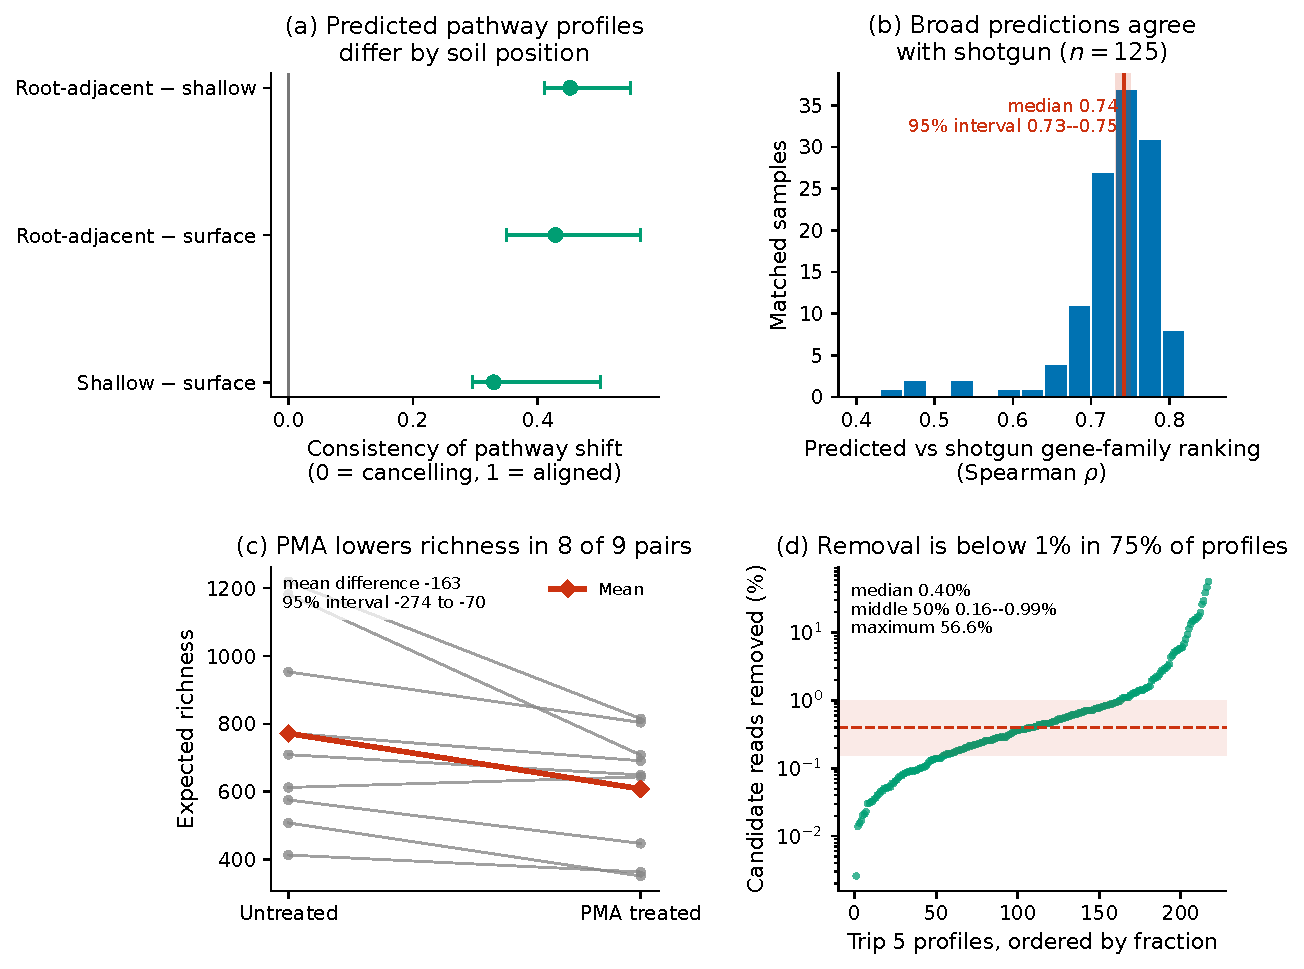
\includegraphics[width=\linewidth]{figures/fig3_function_controls.pdf}
\caption{Predicted function and assay controls. (a) Paired differences in
  predicted pathway profiles. Values approach one when sites shift in the same
  direction and zero when shifts cancel; bars show $95\,\%$ intervals from
  resampling whole sites.
  (b) Agreement between predicted and shotgun-measured gene-family rankings;
  red marks the median and its $95\,\%$ interval. (c) Estimated richness before
  and after PMA treatment; red joins the means and the annotation gives the
  interval for their difference. (d) The fraction of reads assigned to
  candidate contaminants; red marks the median and the range containing the
  middle half of profiles.}
\label{fig:function-controls}
\end{figure}

%% ====================================================================
\section*{Discussion}
%% ====================================================================

\subsection*{The Empty Quarter and global dryland ecology}

The open soils of the Saudi Empty Quarter are organized both across hundreds of
kilometres and within a few centimetres. Taxa replace each other throughout the
landscape, while compartment changes the composition of the community and the balance
between taxa within the sites. Climate, pH, and elemental composition place this
variation in an environmental setting, and predicted pathways suggest that
taxonomic changes carry differences in metabolic potential. The main lesson is
not that one variable controls the desert, but that a hyperarid sand sea
contains a repeatable mosaic at landscape and local scales.

The phylum profile places the Empty Quarter with other hot deserts.
Pseudomonadota, Bacillota, Actinomycetota and Chloroflexota led, and
Acidobacteriota and Verrucomicrobiota, prominent in temperate and agricultural
soils, were minor \cite{makhalanyane2015microbial,fierer2017embracing,
delgadobaquerizo2018global}. The genus level adds a desert-specific signature:
endospore-forming \textit{Domibacillus}, \textit{Bacillus},
\textit{Paenibacillus} and \textit{Lysinibacillus}, together with
\textit{Massilia}, \textit{Microvirga} and \textit{Streptomyces}, supplied
more reads than any other genera.

The change in the geography of the community recurs in desert microbiomes. In the
Empty Quarter, the transect pattern remained at genus and ASV
resolution and across expeditions. Taxon replacement formed $69$--$75\,\%$
of mean dissimilarity, so distant sites usually had different
assemblages rather than smaller subsets of a pool. The replacement has a
recognizable biology: Actinomycetota, Acidobacteriota and Gemmatimonadota
genera such as \textit{Cellulomonas}, \textit{Marmoricola},
\textit{Blastocatella} and \textit{Roseisolibacter} gave way eastward to
Bacillota, with \textit{Bacillus} and genera typical of saline and alkaline
soils gaining most, in the direction in which temperature, humidity and pH
increased. Distance decay
also occurs in Negev soils \cite{bay2020negev}, and Namib dune systems
show habitat-specific community structure across dune zones \cite{ronca2015namib}.
Different primers, distances and soils prevent a merged numerical comparison,
but a presence-based comparison bounds the question of whether the Empty
Quarter is one ecosystem or several. After subsampling every profile to
$8{,}000$ reads and requiring detection in at least $10\,\%$ of profiles, the
western and eastern thirds of the transect shared $267$ of $418$ genera
(Jaccard $0.64$; $0.68$ and $0.83$ for adjacent thirds), and all $50$ leading
genera of either end were detected at the other. The Empty Quarter and a
public Atacama soil pit \cite{horstmann2024atacama} shared $43$ of $397$
genera (Jaccard $0.11$), and only $17$ of the $50$ leading Empty Quarter genera
reached the detection threshold in the Atacama profiles (Supplementary
Section~S9.2). The overlap between the transect ends was therefore six times
the overlap between deserts. Within-desert replacement is strong, but it
reorders a largely shared regional pool; the Empty Quarter behaves as one
regional system with internal structure rather than as several unrelated
ecosystems. Primer, DNA-fraction and depth differences inflate the Atacama
contrast, and all three deserts reject the hypothesis that there is one
representative ``desert soil'' community.

Water was associated with diversity on two scales. Along the
landscape, long-term temperature, rainfall, and humidity were
negatively associated with diversity. After individual rainfall events, by
contrast, richness was highest during the first several days, and the
fitted association then declined. These patterns answer different
questions: the long-term comparison separates sites with different
climate histories, while the pulse model compares rainfall amount and
time before collection. Pulse-reserve theory predicts that rare rainfall
can briefly release water limitation before drying restores it
\cite{noymeir1973desert,schwinning2004pulse}. Rapid cell
resuscitation, solute movement, or improved detection of rare taxa
could produce our pattern; the marker-gene data alone cannot
distinguish them. Direction also varies among deserts. In a public
Atacama gradient, soil humidity was positively associated with Shannon
diversity even after accounting for latitude, longitude, and elevation
(rank correlation $0.68$, $p=0.004$)
\cite{neilson2017significant}. Therefore, water source, evaporation, soil
chemistry, and the range sampled matter more than a global
rule such as ``more water means more diversity''
\cite{coleine2024dryland}.

Physical stratification also occurs, although its direction depends on
scale.  An Atacama pit showed differences in community composition
among depth zones ($p=0.0014$) without a steady increase or decrease
in diversity, and Mojave biocrust communities differ between surface
and subsurface soil
\cite{horstmann2024atacama,pombubpa2020mojave}. The Empty Quarter adds
repeated comparisons of surface, $5$--$10\,\mathrm{cm}$ and root-adjacent
soil. Root-adjacent communities were less even rather than simply poorer, so
fewer taxa carried more reads. This pattern is consistent with a stronger
selective environment near roots: plants change carbon and nutrient supply,
and studies of desert plants have found host- and root-compartment-specific
recruitment \cite{philippot2013roots,eida2018desertplants,
marasco2022namib,maurice2024alula}. Proximity to a root defines this
compartment, so the root is the most likely source of the difference. Because
the host plants were not identified and the soil was root-adjacent rather than
root-attached, the data cannot separate a general root effect from
host-specific recruitment, and they do not show which plant traits matter. The
genus contrasts in Figure~\ref{fig:soil-position}d identify targets for
culture, genome and plant-association studies.

Predicted pathways followed geography and compartment, suggesting
that the taxonomic mosaic carries different metabolic
potential. The dominant predicted biochemistry is aerobic heterotrophy:
respiration through cytochrome $c$ and the biosynthesis of amino acids, fatty
acids and cofactors led the profiles, while carbon-fixation pathways and
Cyanobacteriota were minor. This is the profile expected for an
endospore-rich community that lives on scarce, episodic organic input rather
than on photoautotrophic crusts \cite{makhalanyane2015microbial}. Along the
route, most of the $92$ pathways that changed monotonically were biosynthesis
pathways that increased eastward ($54$ of $63$), including unsaturated
fatty-acid pathways, whereas near roots the supported differences included
carbohydrate degradation and polyamine and thiamin biosynthesis.
Agreement with matched shotgun profiles supports this broad
reading, not measured activity. In the Namib, direct gas uptake, ATP
and respiration measurements showed more than a $30$-fold rise in
hydrogen oxidation after wetting \cite{tribbia2026tracegas}. Our
predictions identify where comparable process measurements are needed.

The relic-DNA experiment addresses DNA that remained accessible after cell
membranes were damaged. PMA treatment reduced the expected richness in $8$ out of $9$
pairs (Figure~\ref{fig:function-controls}c), showing that PMA-sensitive DNA
contributed taxa to these aliquots. PMA does not directly measure viability or
a quantitative relic-DNA fraction \cite{wang2021pma}. The experiment also did
not provide a balanced comparison of the three compartments, so it cannot
show whether PMA-sensitive DNA was more abundant on the surface than below it.

The extraction blanks address a separate low-biomass risk: DNA introduced
during laboratory processing. Candidate contamination was small in most
linked samples, although one profile was strongly affected, and filtering
left all $25$ tracked conclusions unchanged
(Figure~\ref{fig:function-controls}d). This sensitivity supports the reported
patterns for linked profiles, but cannot replace missing or
mismatched controls in the assay \cite{fierer2025controls}. The control design and its
trip-specific limits are reported in Materials and Methods and Supplementary
Section~S2.

\subsection*{A regional framework for the Arabian Peninsula}

Earlier Arabian studies established local habitat-specific patterns. A
groundwater-fed UAE sabkha contained a saline microbial mat, while Saudi
studies examined highland soils, arid locations, biological crusts, and desert
plants \cite{yasir2015elevation,khan2020saudi,aslam2016rainfall,
eida2018desertplants,mckay2016sabkha}. This work revealed local habitat and
plant effects without mapping the open interior. Our survey supplies that
landscape frame and repeated compartment measurements.

The mean pH of $7.986$, measured in a calcium chloride solution, is in the
alkaline range reported for Saudi arid soils \cite{khan2020saudi}. At AlUla, a
plant-created patch of more fertile soil had a different bacterial community
from nearby bare sand; the bare sand was also more alkaline
\cite{maurice2023fertility}. In the Empty Quarter, pH shared substantial
variation with geography rather than replacing it. Plant patches may therefore
modify a broader regional setting.

Regional experiments help interpret compartment and rainfall results.
Around \textit{Rhazya stricta}, the soil compartment had a larger effect than
the simulated rainfall, while crust biomass increased $3$-fold $1$ week after watering
\cite{aslam2016rainfall}. At Jizan and Al Wahbah, the rhizosphere resembled the 
surrounding bulk soil while the root endosphere did not, showing the strongest 
loss of richness and evenness and a composition that tracked host plant 
phylogeny \cite{eida2018desertplants}. Our near-root samples lie in a
compartment Eida et al. did not sample; their lower evenness extends this
local organization outward from the root without identifying a host filter. The rapid
watering result independently shows that an Arabian desert community can
change within days, but its crust-biomass endpoint does not validate our
bacterial-richness curve. Host identity, metabolite exchange, and plant benefit
remain open questions.

The mapped variation makes this survey useful for regional decisions because
a single reference site or compartment could be mistaken for the state of
the wider desert. Saudi Arabia's cloud-seeding programme aims to enhance rainfall
and support ecosystem restoration \cite{saudi_cloud_seeding}. Our rainfall
association suggests a concrete sampling schedule for testing soil-community
change during the first several days after natural or enhanced rainfall, while it
does not predict the effect of cloud seeding. The western Empty Quarter also
contains the Uruq Bani Ma'arid protected area and free-ranging Arabian oryx
\cite{ncw_uruq_bani_maarid}; drought effects on reintroduced oryx show why
habitat condition and climate matter for management \cite{ismail2011oryx}.
Repeated microbial measurements could add soil and vegetation context before
and after habitat restoration, but they are not a measure of oryx health.
For arid agriculture, the survey identifies comparable background sites and
candidate taxa or predicted pathways for later plant trials
\cite{khan2020saudi,eida2018desertplants}. The linked samples, measurements,
sequences and provenance make these comparisons reusable
\cite{rubalkhali_datapaper}; they do not show that a microbial treatment will
improve crops.

\subsection*{Limitations and identifying mechanisms}

Our study primarily measures associations and does not establish
causes. The sites lie on one west--east route, climate changes along
that route, and every expedition traveled in the same direction. The
shared route links location to collection order, time of day and
changes during travel, and the study design cannot separate their
individual effects from geography. Independent or crossing transects
with randomized route direction would separate these alternatives, but they
are difficult in the roadless dune interior. The field team must use long,
logistically feasible off-road traverses through an isolated landscape, which
limits route randomization and simultaneous crossing surveys
\cite{edgell2006arabian}. A next practical design could reverse the direction of travel
 between expeditions, add shorter crossing transects where terrain
allows, and leave autonomous soil sensors at selected sites.

Several measurements needed to test ecological explanations are
missing. Air measurements are not soil microclimate, and XRF measures
total elements rather than soluble ions, conductivity or osmotic
stress \cite{elmoatassem2025pxrf}. The rainfall model used gridded
daily estimates and collection dates, not soil moisture or collection
time. Rainfall was too rare and uneven for the omission of one expedition to
be a meaningful stability test; the randomization test instead shifted
the timing of the rainfall observed within each expedition. Its
first-several-days window remains an association, and models that
allowed more complex geographic change weakened the evidence.
Event-triggered sampling before and after storms, moisture sensors and
watering experiments are needed to measure response time and test a
mechanism. Root identity, root distance, carbon, texture and plant
performance would likewise separate plant effects from shared habitat.

Shotgun metagenomics could recover genes without biases caused by $16$S
primers or by bacteria that carry different numbers of $16$S gene
copies. It could also link functions to genomes, resolve strains, and
include archaea, fungi and viruses. It would test whether predicted
pathways occur in the local gene pool, but DNA still measures
potential. Transcripts, proteins, metabolites, cell counts and process
rates are needed to show activity, while manipulations remain
necessary for causation \cite{ray2023chemosynthesis}.

Control coverage was uneven. Purified-DNA standards do not test
extraction, whole-cell standards do, Trip~$4$ had no field-based positive
or negative control (a PCR-stage-only positive control was run, and its PCR
blank and no-template control were not sequenced), and
Trip~$5$ controls used shotgun rather than $16$S. Linked
extraction blanks could train the contaminant sensitivity for
Trips~$4$ and $5$ only. Future work should sequence extraction and PCR blanks
with every batch, use positive standards that enter at the same stage
as the biological samples, and retain DNA concentrations. Stable
filtered results cannot substitute for missing controls.

\subsection*{Conclusions}

The Empty Quarter is a structured microbial landscape. Bacterial
assemblages turn over across the sand sea, nearby compartments
differ in composition and evenness, environmental gradients track the
broad pattern, and recent rainfall was associated with a short rise in
richness. Predicted metabolic potential also changes with geography
and compartment. These findings extend recurring dryland principles
to the world's largest continuous sand desert while showing that the
direction of diversity--environment associations remains local. The
survey provides a regional reference and a set of testable hypotheses
bounded by relic-DNA and contamination checks.

%% ====================================================================
\section*{Materials and Methods}
%% ====================================================================

\subsection*{Field design and sample description}
We sampled a transect through the Empty Quarter during
expeditions on March $17$--$20$, $2023$ (T1), July $14$, $2023$ (T2),
February $17$--$21$, $2024$ (T3), August $19$--$21$, $2024$ (T4), and
October $12$--$15$, $2025$ (T5). Each sampling campaign covered $60$ sites, while extreme heat restricted T2 to $8$
sites. At each site and
visit, we sampled bulk surface soil ($0\,\mathrm{cm}$), bulk subsurface soil
($5$--$10\,\mathrm{cm}$) and subsurface soil referred to as ``root-adjacent'' collected near plant roots ($5$--$10\,\mathrm{cm}$), collecting three replicates per compartment. Sampling initially targeted the
rhizosphere, but most plants were so desiccated that root-attached soil could
not be obtained; we therefore collected soil as close to the root as possible,
which in some cases included root-attached soil. We call this compartment
``root-adjacent soil'' rather than rhizosphere because soil was not
consistently attached to roots. Soil was placed in sterile tubes by
scooping directly with the tube or with a sterile plastic spoon. Samples were
kept at $-20\,^{\circ}\mathrm{C}$ in a portable freezer during each expedition
and transferred to $-80\,^{\circ}\mathrm{C}$ in the laboratory.

Here, a profile means one quality-controlled $16$S amplicon library and its counts
for exact bacterial $16$S amplicon sequences, which we call amplicon sequence variants
(ASVs). Analyses that required repeat visits focused on sites $1$--$60$ and used
$1{,}227$ profiles. Four locations sampled only during Trip~$1$ contributed $10$ additional
profiles. We retained them for description but excluded them from repeated-site
analyses because later expeditions could not revisit these sites. Supplementary
Table~S1 reports the samples used in each analysis.

\subsection*{Amplicon processing}
Between $0.9$ and $1.2\,\mathrm{g}$ of soil was extracted with QIAGEN
PowerLyzer PowerSoil or DNeasy PowerSoil Pro kits. Samples were homogenized
with a PowerLyzer~$24$, processed manually or with a QIACube Connect, and
eluted in $50\,\mu\mathrm{L}$. The V3--V4 region of the $16$S rRNA gene was amplified with
the Bakt\_341F (\texttt{CCTACGGGNGGCWGCAG}) and Bakt\_785R
(\texttt{GACTACHVGGGTATCTAATCC}) primers \cite{klindworth2013primers},
both carrying Illumina overhang adapters. First-round PCR used TaKaRa Ex
Taq DNA Polymerase (catalogue no.\ RR001B) in $50\,\mu\mathrm{L}$ reactions
containing $5\,\mu\mathrm{L}$ of extracted DNA and $0.4\,\mu\mathrm{M}$ of
each primer: $95\,^{\circ}\mathrm{C}$ for $3\,\mathrm{min}$; $30$ cycles of
$95\,^{\circ}\mathrm{C}$ for $30\,\mathrm{s}$, $63\,^{\circ}\mathrm{C}$ for
$30\,\mathrm{s}$ and $72\,^{\circ}\mathrm{C}$ for $1\,\mathrm{min}$; and a
final $72\,^{\circ}\mathrm{C}$ extension for $6\,\mathrm{min}$. Products
were checked on a $1\,\%$ agarose gel; samples with an amplicon of the expected
size (about $500\,\mathrm{bp}$) were indexed, samples without a visible product
were re-amplified with more DNA input, and samples that still failed were
re-extracted.


Dual indices and Illumina adapters were added in a second-round
PCR with the QIAGEN Multiplex PCR Kit (catalogue no.\ 206143) following the
Illumina $16$S protocol \cite{illumina16S}: $94\,^{\circ}\mathrm{C}$ for
$15\,\mathrm{min}$; $8$ cycles of $94\,^{\circ}\mathrm{C}$ for
$30\,\mathrm{s}$, $55\,^{\circ}\mathrm{C}$ for $30\,\mathrm{s}$ and
$72\,^{\circ}\mathrm{C}$ for $30\,\mathrm{s}$; and $72\,^{\circ}\mathrm{C}$
for $5\,\mathrm{min}$. Indexed libraries were purified with Agencourt AMPure
XP beads, quantified with the Qubit high-sensitivity double-stranded DNA
assay, sized on an Agilent TapeStation~$4200$ (D5000 ScreenTape), and pooled
by concentration and size. Amplicon pools were sequenced on an Illumina
NovaSeq~$6000$ on an SP flow cell with a $500$-cycle reagent kit to generate
$2\times250$-bp paired-end reads. Sample processing and library preparation
were performed in the PI's laboratory and sequencing was conducted at the
Bioscience Core Lab at KAUST.


Reads were processed with
nf-core/Ampliseq v2.14.0 \cite{nfcore, ampliseq}. We used DADA2 to infer exact
amplicon sequence variants (ASVs)
and SILVA~$138.2$ \cite{silva} to assign taxonomy. The complete count table retained
all $351{,}472$ ASVs and $24$ control profiles from the Trip~$5$ sequencing run
($18$ extraction blanks and $6$ no-template PCR controls). We excluded these controls and $10$
biological profiles below $1{,}000$ reads, leaving $1{,}237$ profiles. Positive
standards, PCR blanks and no-template controls were evaluated in their
source-specific data and were never ecological profiles. The unfiltered biological table was
the primary analysis input.

\subsection*{Assay controls and sensitivity analyses}

We followed low-biomass guidance by analysing each control according to the
stage it tested \cite{fierer2025controls}. $17$ sequenced extraction blanks
could be linked by extraction day to $217$ Trip~$5$ profiles. We pooled
these blanks and marked an ASV as a candidate when it appeared in at least $2$
blanks and was more prevalent in blanks than in biological samples in a
one-sided Fisher test ($p<0.1$). The $351$ candidates were removed only from
their linked profiles in a filtered copy used to test sensitivity. The
remaining Trip~$5$ extraction blank and the $6$ no-template controls had no
extraction-day link and were characterized without being used to identify
candidates. The $6$ Trip~$4$ extraction blanks were sequenced on a separate run
and denoised from the raw reads with the same pipeline; screened in the same way
against the $95$ Trip~$4$ profiles linked through the extraction-batch map, they
gave $7$ candidate ASVs (four unassigned at genus level, \textit{Nesterenkonia},
\textit{Brevibacterium} and \textit{Alcaligenes}) whose removal changed a median
of $0.00\,\%$ of reads per linked profile (maximum $14.3\,\%$; $0.14\,\%$ pooled).
The Trip~$4$ PCR blank and no-template control
were not sequenced because their index pairs conflicted with biological samples
from Trips~$1$--$3$ on that run. No-template controls and PCR blanks contain the
amplification reagents but no sample, so they test a later laboratory step;
they were kept separate because their biological batch links were incomplete. Positive
standards were used only to assess
expected-taxon recovery and whether their expected taxa appeared in other
samples. Supplementary Section~S2 gives the
trip-specific products, assay stages and remaining coverage gaps.


For the contamination sensitivity, we removed the $351$ Trip~$5$ candidate ASVs
only from the $217$ linked Trip~$5$ profiles and the $7$ Trip~$4$ candidates only
from the $95$ linked Trip~$4$ profiles. Trip~$5$ candidate sequences comprised
$2.19\,\%$ of reads overall and a median of $0.40\,\%$ per profile
(interquartile range, $0.16$--$0.99\,\%$); $1$ profile contained
$56.60\,\%$ candidate reads (Figure~\ref{fig:function-controls}d). Every
filtered profile remained above $25{,}000$ reads. We repeated $25$ geographic,
environmental and compartment conclusions with this filtered copy; all
retained the same disposition as in the unfiltered primary analysis.

\subsection*{Relic-DNA removal and viability assessment}
To distinguish DNA from intact, viable cells from total environmental DNA
(including relic DNA), soil samples from $3$ Trip~$5$ sites were subjected to
PMAxx-based viability treatment, following established protocols for relic-DNA
removal from soil matrices \cite{carini2017relic,sun2023}. For each site,
$3$ independent biological replicates were prepared as soil slurries by
homogenizing soil in sterile phosphate-buffered saline (PBS, pH $7.4$) at a
$1$:$10$ (w/v) ratio. Each replicate was partitioned into two aliquots:
``treated'' (T), used to quantify DNA from intact cells, and ``untreated''
(U), serving as a total-DNA baseline, yielding $9$ matched treated/untreated
pairs across the $3$ sites. PMAxx dye (Biotium, Hayward, CA, USA) was added
to treated aliquots at a final concentration of $50\,\mu\mathrm{M}$, followed
by a $10$-minute dark incubation. Samples were photoactivated by exposure to a
$450\,\mathrm{nm}$ LED lamp for $35$ minutes, with tubes positioned on a white
reflective surface $15$--$20\,\mathrm{cm}$ from the light source and rotated
at $15$-minute intervals. Immediately after photoactivation, all samples were
stored at $-20\,^{\circ}\mathrm{C}$ until DNA extraction, which was performed
on $860\,\mu\mathrm{L}$ of each sample using the DNeasy PowerSoil Pro Kit
(QIAGEN). $16$S rRNA amplicon libraries from these samples were sequenced on
an Illumina NovaSeq~$6000$ with the same $500$-cycle kit and $2\times250$-base
paired-end configuration as the main sample set.

Propidium monoazide (PMA) enters cells with damaged membranes and prevents
their exposed DNA from being amplified \cite{wang2021pma}. We compared $9$
matched treated and untreated Trip~$5$ aliquot pairs. We calculated Hurlbert
expected richness at $123{,}897$ reads, the minimum depth among the $18$
libraries, without random subsampling, and calculated Shannon diversity at
full depth. Exact two-sided paired Wilcoxon tests compared the two endpoints;
$99{,}999$ bootstrap samples of the matched aliquots gave uncertainty for
their mean differences (seed $20260805$). Expected richness was lower after
treatment in $8$ pairs
(mean treated-minus-untreated difference, $-163.3$ taxa; $95\,\%$
paired-aliquot bootstrap interval, $-274.0$ to $-69.8$; exact paired
$p=0.00781$; Figure~\ref{fig:function-controls}c). This experiment measures a
PMA-sensitive richness difference in these aliquots. It does not estimate cell
viability, a survey-wide relic-DNA fraction, or a difference among the $3$
surveyed compartments. Supplementary Sections~S2 and~S7.3 give the control
provenance, quality checks and uncertainty calculations.

\subsection*{Environmental measurements}
At each site visit we recorded air temperature and, where available, atmospheric pressure and relative humidity. We retained confirmed values and excluded one
out-of-range measurement. We used these measurements in a secondary analysis (Supplementary Section~S7.1) where we 
% related this collection weather to diversity after accounting for campaign and for a geographic pattern that could change steadily or change its rate smoothly and reverse once along the route. Uncertainty estimates kept repeated measurements from the same site together.
averaged each diversity measure within site and campaign, and tested its association with each variable.
We included campaign and position along the transect (linear and quadratic terms) as covariates, with standard errors clustered by site to account for repeated visits. The nine tests were corrected together with the Benjamini--Hochberg method.
%These are air, not soil, measurements.

We obtained site-specific monthly air temperature, total rainfall, and relative
humidity from the Open-Meteo historical API resource
\cite{openmeteo}. Each site had $49$ complete months from January $2022$ to
January $2026$. We averaged climate and the three diversity measures within each
site, then used the $60$ sites for Spearman correlation. We corrected the $9$ climate--diversity tests together for multiple testing with the Benjamini--Hochberg
method. For abundance,
we selected the $200$ genera with the largest mean abundance among those detected
in at least $20\,\%$ of profiles. We added $0.5$ to every count so that zero counts
could enter the logarithm, then calculated
each genus's log ratio to the geometric mean abundance across all genera. This
centred-log-ratio (CLR) transformation compares taxa within a relative
composition instead of treating read counts as absolute abundances. We
averaged the transformed abundances by site. We corrected the $600$ climate--genus tests together in a second set.


We measured pH in $767$ archived soil samples from all campaigns. Dry
soil below $2$~mm was mixed with $0.01$~M CaCl$_2$ at $1$:$2.5$ mass-to-volume and
measured with an accumet AB315. We required a valid date and range, recorded
calibration, an electrode slope of $95$--$102\,\%$, and a pH $10$ buffer read-back of
$9.9$--$10.1$. In total, $712$ measurements passed and $702$ matched ecology profiles, and
we did not impute missing values. We averaged matched values within site,
campaign and compartment. The composition test added pH after expedition,
compartment and site and randomly rearranged the remaining variation within sites
$999$ times. We compared
the transect result before and after pH adjustment in the same samples.

Laboratory XRF covered $725$ archived-soil specimens. We retained $11$ elements
detected in at least $75\,\%$ of specimens, transformed values as $\log(1+x)$,
placed them on a common scale within each expedition and combined them by
principal component analysis. This method constructs weighted combinations of
the elements; the first component captures the largest shared change. We tested
whether this component explained bacterial composition beyond expedition,
compartment and site, using $999$ random rearrangements within sites. Changes to the
included taxa and the treatment of zero values tested sensitivity. XRF
describes total elements, not salinity or soluble ions
\cite{elmoatassem2025pxrf}. Supplementary Sections~S2--S4 give the laboratory
quality checks, coverage and complete models.

\subsection*{Short-term rainfall response}

We obtained daily precipitation for each site from the versioned NASA POWER
\texttt{PRECTOTCORR} resource \cite{nasa_power_2024}; Open-Meteo provided an
independent rainfall dataset for comparison. We excluded the sampling date because
collection times were unavailable. Technical replicates were averaged within
$617$ site, expedition, and compartment groups.

We represented a temporary response by weighting rainfall over the $60$ complete
days before collection. For rainfall $r_{i,d}$ at site observation $i$ and $d$
complete days before collection, the pulse score for a possible peak at day
$p$ was
\[
x_i(p)=\sum_{d=1}^{60}r_{i,d}(d/p)\exp(1-d/p).
\]
The weight rises to one at $d=p$ and then declines. We searched
$p=0.5,1.0,\ldots,30.0$ days for expected
richness at $25{,}000$ reads, Shannon diversity and normalized evenness. Each
model allowed each site and compartment to have its own baseline, each
expedition to have its own mean, and longitude and collection day to have
separate steady trends within each expedition.

To account for choosing the strongest result from many peaks and diversity
measures, we shifted the full $60$-day rainfall sequence in a circle $19{,}999$ times,
independently within each expedition (seed $20260804$). Each shifted dataset
retains the amount, rarity and spatial pattern of rainfall but changes its timing
relative to collection. We used a one-sided test for the stated prediction of
a positive pulse and also report a two-sided test that allows either direction;
both tests cover the complete search. Confidence intervals for the selected
effect used sandwich covariance clustered by site. We resampled whole
sites $9{,}999$ times (seed $20260805$) to estimate the share of remaining variation
explained by rain and the uncertainty in peak selection. Supplementary
Section~S7 describes these calculations and the comparison of rainfall
datasets. Additional analyses changed the rainfall dataset, contaminant
filtering, pH adjustment, and geographic trend and included samples. To check the
assumed pulse shape, we fitted rainfall from $1$, $2$, $3$--$4$, $5$--$7$,
$8$--$14$, $15$--$30$ and $31$--$60$ complete days before collection
together for each rainfall dataset, with site-clustered uncertainty. We also
used future rainfall as a negative control. Supplementary Section~S7 gives these
results, and the exact reproducibility manifests.

\subsection*{Community, diversity and spatial analyses}
To compare richness at the same sequencing depth, we calculated Hurlbert's
expected richness: the number of taxa expected if each profile contributed
$25{,}000$ reads. We fixed this depth before analysis as a common
standardization depth near the $5$th percentile of library size (median
$382{,}432$ reads per profile), so that expected richness is comparable across
profiles while $95\,\%$ of them are retained; the $60$ profiles with fewer reads
($55$ of them core profiles) contributed no expected-richness value, and no
profile was discarded on this basis (Supplementary Section~S2). We did not use
rarefaction curves to select the depth; Shannon diversity used full depth. We averaged profiles within
site, expedition and compartment before paired compartment comparisons. Means and
intervals came from repeatedly sampling whole sites with replacement. We drew
$1{,}000{,}000$ whole-site bootstrap samples (seed $20260723$), keeping all repeated
observations from one site together. We corrected each family of $3$
contrasts. An additional evenness analysis used
$H/\log(E[S_{25k}])$, where $H$ is Shannon diversity and $E[S_{25k}]$ is
expected richness at $25{,}000$ reads. This measures abundance balance relative to
common-depth richness; it is not conventional Pielou evenness.
Supplementary Section~S5.2 gives campaign-specific contrasts and correction
families.

For composition, we combined replicate counts within expedition, site and
compartment. We selected the $200$ most abundant genera among those detected in at
least $20\,\%$ of profiles, added $0.5$ to every count to handle zeros, and used the
CLR transformation defined above \cite{gloor2017compositional}. This small
addition is called a pseudocount. The paired test
used $170$ complete three-compartment comparisons across $60$ sites. Pairwise tests
randomly reversed the direction of each within-pair difference while keeping
all observations from a site together. Alternative taxon sets, treatments of
zero counts and expedition omissions tested sensitivity.

For broad spatial structure, we retained core-site groups with at least $2{,}000$
reads, removed the CLR mean for each expedition and compartment, and averaged
within site. The route model allowed both steady change from west to east and a
smooth change in rate that could reverse once, represented by straight-line and
squared-location terms. It used the
same $200$ genera and $999$ random rearrangements of whole sites. Taxon sets, trend
shapes and expedition omissions tested sensitivity. To quantify sampling
uncertainty in the explained share, we removed each of the $60$ sites in turn,
refitted the model, calculated the delete-one-site jackknife standard error,
and formed a $95\,\%$ $t$ interval with $59$ degrees of freedom.

To measure distance decay within each compartment, we removed the campaign
mean from the CLR composition at each of the $60$ sites and related Aitchison
dissimilarity to distance. We randomly reassigned location labels to whole
sites $9{,}999$ times across all compartments, so the $1{,}770$ pairs of sites were
not treated as independent observations. For comparisons based only on whether
a taxon was present, we pooled counts within site and compartment and randomly
subsampled each pooled sample to the same $12{,}865$ reads (seed $20260728$). We partitioned Sørensen
dissimilarity into taxon replacement and nestedness
\cite{baselga2010partition}. Delete-one-site jackknife intervals for the
distance slopes and mean replacement shares removed every pair involving the
omitted site.

Supplementary Section~S5 gives the spatial prediction, ASV-resolution and
dispersion diagnostics.

To describe the taxa behind these patterns, we summed ASV counts per phylum,
class and genus and expressed them as shares of total reads per profile across
the $1{,}227$ core profiles, overall and by compartment and by transect third
($20$ sites each, ordered by route position). For the $200$ genera of the
route model, we correlated the site-level CLR values (expedition-by-compartment
means removed) with route position (Spearman; Benjamini--Hochberg over $200$
tests) and estimated the east-minus-west difference in mean CLR with a
delete-one-site jackknife interval. To compare within-transect with
between-desert differences under one rule, we subsampled every Empty Quarter
profile and every Atacama pit profile \cite{horstmann2024atacama} $20$ times to
$8{,}000$ reads (seed $20260903$), called a genus detected in a set when it
occurred in at least $10\,\%$ of subsampled profiles, and computed Jaccard
overlaps between transect thirds and between the Empty Quarter and the pit
(all depths, and $2.5$--$10$~cm only). This comparison uses presence only; it
does not correct for the different primers (V3--V4 versus V4) or DNA fractions
(total versus intracellular). Site-level pH and climate means were correlated
with route position to state the direction of the gradients. These summaries
are descriptive and add no claim to the tracked conclusions
(\path{analysis/v3/taxon_context/}).

\subsection*{Predicted functional potential and shotgun comparison}

PICRUSt2 v2.4.1 predicted KEGG Ortholog groups and MetaCyc pathways from the ASV
tables \cite{douglas2020picrust2}. We matched $1{,}227$ core-site profiles, summed
replicates within expedition, site and compartment, and ranked pathways detected
in at least $20\,\%$ of groups. The primary analysis used the $200$ with largest
mean abundance, a $0.5$ pseudocount and CLR coordinates. For geography, we
removed expedition-by-compartment means and tested the route model that allowed
the rate of change to vary smoothly and reverse once, using $9{,}999$ random
rearrangements of whole sites. The pathway geography interval used the same
delete-one-site jackknife and $95\,\%$ $t$ interval as the taxonomic route
model. For compartment,
we expressed each complete three-compartment comparison relative to its own mean
and then averaged within site. The overall test randomly reassigned compartment
labels within sites; pairwise tests randomly reversed the site-level
differences. We corrected $3$ profile comparisons together and $600$ pathway
comparisons together. Pathway sets, pseudocounts and expedition omissions
tested sensitivity. To describe the dominant predicted metabolism, we
expressed each pathway as a share of predicted pathway abundance per profile,
averaged across the $1{,}227$ core profiles, and grouped pathways by keywords
in their MetaCyc descriptions into biosynthesis, degradation or utilization,
energy and central metabolism, and other; the rules and the ranks of the
carbon-fixation pathways are archived with the results.

For each predicted profile, the weighted nearest-sequenced-taxon index (NSTI)
summarized the distance between its ASVs and sequenced reference genomes. A
smaller value means that the prediction requires less extrapolation. For an
empirical comparison, we matched PICRUSt2 and shotgun-derived abundance for
$3{,}471$ KEGG Ortholog gene families in $125$ samples, calculated a Spearman rank
correlation within each sample, and also correlated the two community-average
profiles. The shotgun data were not generated for this paper: they come from a
separate, ongoing metagenomic study of the same expeditions (BioProject
\todo{BioProject accession}), in which $125$ shotgun libraries from Trip~$5$
matched $16$S profiles in this survey. That study's assembly, binning,
dereplication and eggNOG-mapper v2.1.12 annotation of the genome catalogue
produced the CoverM genome-abundance profiles and KEGG Ortholog annotations we
reused here; its results will be reported separately. Supplementary Section~S8 reports the uncertainty method and the
limits of pathway and marker-gene predictions.

\subsection*{Cross-desert contextual analysis}

We compared effects in $2$ public Atacama datasets without merging their ASV
counts. In QIITA study $10360$ (PRJEB17617), technical replicates were averaged
within $16$ sites; Spearman correlations related diversity to soil humidity
before and after adjustment for latitude, longitude and elevation. In
PRJEB39249, $62$ intracellular-DNA profiles were aggregated to $23$ sampled depths.
Three depth zones were compared in $200$-genus CLR coordinates with $9{,}999$ label
rearrangements; diversity was averaged after subsampling each profile $100$ times
to $8{,}000$ reads.
Supplementary Section~S9 gives the upstream processing and comparison limits.

\subsection*{Sensitivity analyses and reproducibility}
To test whether sequencing depth or recorded extraction method explained the
Shannon compartment differences, we fitted a Gaussian generalized estimating
equation with sequencing depth, expedition and extraction protocol. This
regression method accounts for repeated observations from the same site.
We treated these models as robustness checks because extraction protocol and
laboratory batch were incompletely recorded and partly linked to expedition.
The companion data descriptor covers the field, specimen, amplicon,
environmental, XRF and knowledge-graph resources \cite{rubalkhali_datapaper}.
Inputs, scripts, machine-readable results, random seeds and checksums are
maintained in the dedicated reproducibility repository at
\url{https://github.com/bio-ontology-research-group/empty-quarter-ecology-reproducibility}.
The repository links each analysis to its exact input, machine-readable result,
random seed and checksum, and links shared data products to the companion
resource. Public deposition of the ecology package and upstream amplicon, PMA,
shotgun-read and genome resources remains a submission requirement.

\subsection*{Software}
Amplicon reads were processed with nf-core/Ampliseq v2.14.0 (Nextflow; DADA2
and SILVA~$138.2$) on the KAUST Ibex cluster, where the eggNOG-mapper v2.1.12
annotation of the shotgun genome catalogue also ran. All statistical analyses
were run on a Linux workstation in Python $3.11.14$ with pandas $2.2.3$, NumPy
$2.1.3$, SciPy $1.14.1$, statsmodels $0.14.6$, scikit-learn $1.5.2$, scikit-bio
$0.7.3$ and Biopython $1.84$; PICRUSt2 v2.4.1 predicted functional potential.
Figures were drawn with Matplotlib $3.9.4$ (FreeType $2.14.3$). The complete
environment is pinned as a conda lock file with hashed pip requirements in the
reproducibility repository, and every reported number is regenerated from the
committed inputs by the repository's tests. We used Claude (Anthropic) to
assist with writing analysis code and with editing the manuscript; all
analyses, results and claims were checked and verified by the authors.

\section*{Funding}
SMA was supported by the Fonds National de la Recherche (FNR), Luxembourg
(Project Ref.\ 18047750).
%% TODO (Robert): add the KAUST and any other grant numbers supporting this work.

%% ====================================================================
\bibliography{sample}

\end{document}
